\documentclass{beamer}
\usepackage[utf8]{inputenc}
\usepackage{graphicx, epsfig}
\usepackage{amsmath,mathrsfs,amsfonts,amssymb}
\usepackage{floatflt}
\usepackage{epic,ecltree}
\usepackage{mathtext}
\usepackage{fancybox}
\usepackage{fancyhdr}
\usepackage{multirow}
\usepackage{enumerate}
\usepackage{epstopdf}
\usepackage{multicol}
\usepackage{algorithm}
\usepackage[noend]{algorithmic}
\usepackage{tikz}
\usepackage{blindtext}
\usetheme{default}%{Singapore}%{Warsaw}%{Warsaw}%{Darmstadt}
\usecolortheme{default}

\setbeamerfont{title}{size=\Huge}
\setbeamertemplate{footline}[page number]{}

\setbeamertemplate{section in toc}[sections numbered]


\makeatletter
\newcommand\HUGE{\@setfontsize\Huge{35}{40}}
\makeatother    

\setbeamerfont{title}{size=\HUGE}
\beamertemplatenavigationsymbolsempty

% latin bold lower
\newcommand{\ba}{\mathbf{a}} 
\newcommand{\bc}{\mathbf{c}} 
\newcommand{\be}{\mathbf{e}} 
\newcommand{\bh}{\mathbf{h}} 
\newcommand{\bp}{\mathbf{p}} 
\newcommand{\bt}{\mathbf{t}} 
\newcommand{\bs}{\mathbf{s}} 
\newcommand{\bu}{\mathbf{u}} 
\newcommand{\bv}{\mathbf{v}} 
\newcommand{\bw}{\mathbf{w}} 
\newcommand{\bx}{\mathbf{x}} 
\newcommand{\by}{\mathbf{y}} 
\newcommand{\bz}{\mathbf{z}} 

% latin bold upper
\newcommand{\bA}{\mathbf{A}} 
\newcommand{\bB}{\mathbf{B}} 
\newcommand{\bC}{\mathbf{C}} 
\newcommand{\bI}{\mathbf{I}} 
\newcommand{\bL}{\mathbf{L}} 
\newcommand{\bM}{\mathbf{M}} 
\newcommand{\bQ}{\mathbf{Q}} 
\newcommand{\bT}{\mathbf{T}} 
\newcommand{\bU}{\mathbf{U}} 
\newcommand{\bV}{\mathbf{V}} 
\newcommand{\bW}{\mathbf{W}} 
\newcommand{\bX}{\mathbf{X}} 
\newcommand{\bY}{\mathbf{Y}} 
\newcommand{\bZ}{\mathbf{Z}} 

% latin cal upper
\newcommand{\cG}{\mathcal{G}} 
\newcommand{\cL}{\mathcal{L}} 
\newcommand{\cN}{\mathcal{N}} 
\newcommand{\cS}{\mathcal{S}} 
\newcommand{\cT}{\mathcal{T}} 
\newcommand{\cW}{\mathcal{W}} 
\newcommand{\cX}{\mathcal{X}} 
\newcommand{\cZ}{\mathcal{Z}} 

% latin bb upper
\newcommand{\bbE}{\mathbb{E}} 
\newcommand{\bbI}{\mathbb{I}} 
\newcommand{\bbP}{\mathbb{P}} 
\newcommand{\bbR}{\mathbb{R}} 

% greek bold lower
\newcommand{\bepsilon}{\boldsymbol{\epsilon}} 
\newcommand{\btheta}{\boldsymbol{\theta}} 
\newcommand{\blambda}{\boldsymbol{\lambda}} 
\newcommand{\bpi}{\boldsymbol{\pi}} 
\newcommand{\bmu}{\boldsymbol{\mu}} 
\newcommand{\bsigma}{\boldsymbol{\sigma}} 
\newcommand{\bphi}{\boldsymbol{\phi}} 

% greek bold upper
\newcommand{\bSigma}{\boldsymbol{\Sigma}} 

\DeclareMathOperator*{\argmin}{arg\,min}
\DeclareMathOperator*{\argmax}{arg\,max}

\newcommand{\createdgmtitle}[1]{\title[\hbox to 56mm{Deep Generative Models  \hfill\insertframenumber\,/\,\inserttotalframenumber}]
	{Deep Generative Models \\ {\Huge Lecture #1}}
	\author{Roman Isachenko}
	\institute{
\includegraphics[width=0.5cm]{../utils/ozonmasterslogo} \large{Ozon Masters}}
	\date{Spring, 2022}
}

\newcommand\myfootnote[1]{%
  \tikz[remember picture,overlay]
  \draw (current page.south west) +(1in + \oddsidemargin,0.5em)
  node[anchor=south west,inner sep=0pt]{\parbox{\textwidth}{%
      \rlap{\rule{10em}{0.4pt}}\raggedright\scriptsize \textit{#1}}};}

\newcommand\myfootnotewithlink[2]{%
  \tikz[remember picture,overlay]
  \draw (current page.south west) +(1in + \oddsidemargin,0.5em)
  node[anchor=south west,inner sep=0pt]{\parbox{\textwidth}{%
      \rlap{\rule{10em}{0.4pt}}\raggedright\scriptsize\href{#1}{\textit{#2}}}};}
      
\AtBeginSection[]
{
	\begin{frame}{Outline}
		\tableofcontents[currentsection,subsectionstyle=hide]
	\end{frame}
}
\AtBeginSubsection[]{
	\begin{frame}{Outline}
		\tableofcontents[currentsection,currentsubsection]
	\end{frame}
}
\createdgmtitle{11}
%--------------------------------------------------------------------------------
\begin{document}
%--------------------------------------------------------------------------------
\begin{frame}[noframenumbering,plain]
%\thispagestyle{empty}
\titlepage
\end{frame}
%=======
\begin{frame}{Recap of previous lecture}
		\begin{block}{WGAN objective}
			\vspace{-0.5cm}
			\[
				\min_{G} W(\pi || p) = \min_{G} \max_{\bphi \in \boldsymbol{\Phi}} \left[ \bbE_{\pi(\bx)} f(\bx, \bphi)  - \bbE_{p(\bz)} f(G(\bz), \bphi )\right].
			\]
			\vspace{-0.5cm}
		\end{block}
		\begin{itemize}
			\item Function~$f$ in WGAN is usually called $\textit{critic}$.
			\item If parameters $\bphi$ lie in a compact set $\boldsymbol{\Phi} \in [-0.01, 0.01]^d$ then $f(\bx, \bphi)$ will be $K$-Lipschitz continuous function. 
		\end{itemize}
		\begin{block}{Gradient penalty}
			\vspace{-0.7cm}
			\[
				W(\pi || p) = \underbrace{\bbE_{\pi(\bx)} f(\bx)  - \bbE_{p(\bx)} f(\bx)}_{\text{original critic loss}} + \lambda \underbrace{\bbE_{U[0, 1]} \left[ \left( \| \nabla_{\hat{\bx}} f(\hat{\bx}) \|_2 - 1 \right) ^ 2\right]}_{\text{gradient penalty}}.
			\]
			\vspace{-0.7cm}
		\end{block}
		Samples $\hat{\bx}_t = t \bx + (1 - t) \by$ with $t \in [0, 1]$ are uniformly sampled along straight lines between pairs of points: $\bx$ from the data distribution $\pi(\bx)$ and $\by$ from the generator distribution $p(\bx | \btheta)$.
		\myfootnote{
		\href{https://arxiv.org/abs/1701.07875}{Arjovsky M., Chintala S., Bottou L. Wasserstein GAN, 2017} \\
		\href{https://arxiv.org/abs/1704.00028}{Gulrajani I. et al. Improved Training of Wasserstein GANs, 2017} }
\end{frame}
%=======
\begin{frame}{Recap of previous lecture}
	\vspace{-0.3cm}
	\[
		f(\bx, \bphi) = \bW_{K+1} \sigma_K (\bW_K \sigma_{K-1}(\dots \sigma_1(\bW_1 \bx) \dots)).
	\]
	\vspace{-0.3cm}
	\begin{itemize}
		\item $\sigma_k$ is a pointwise nonlinearities. We assume that $\| \sigma_k \|_L = 1$ (it holds for ReLU).
		\item $\mathbf{g}(\bx) = \bW \bx$ is a linear transformation ($\nabla \mathbf{g}(\bx) = \bW$).
		\[
			\| \mathbf{g} \|_L = \sup_\bx \| \nabla \mathbf{g}(\bx) \|_2 = \|\bW\|_2.
		\]
	\end{itemize}
	\vspace{-0.5cm}
	\begin{block}{Critic spectral norm}
		\vspace{-0.5cm}
		\[
			\| f \|_L \leq \| \bW_{K+1}\|_2 \cdot \prod_{k=1}^K  \| \sigma_k \|_L \cdot \| \bW_k \|_2 = \prod_{k=1}^{K+1} \|\bW_k\|_2.
		\]
		\vspace{-0.5cm}
	\end{block}
	\begin{block}{Spectral Normalization GAN}
	If we replace the weights in the critic $f(\bx, \bphi)$ by $\bW^{SN}_k = \bW_k / \|\bW_k\|_2$, we will get $\| f\|_L \leq 1.$ \\
	\end{block}
	 Power iteration approximates the value of $\|\bW\|_2$.
	\myfootnotewithlink{https://arxiv.org/abs/1802.05957}{Miyato T. et al. Spectral Normalization for Generative Adversarial Networks, 2018}
\end{frame}
%=======
\begin{frame}{Recap of previous lecture}
	\vspace{-0.3cm}
	\begin{block}{f-divergence minimization}
		\vspace{-0.3cm}
		\[
			D_f(\pi || p) = \bbE_{p(\bx)}  f\left( \frac{\pi(\bx)}{p(\bx)} \right) \rightarrow \min_p.
		\]
		Here $f: \bbR_+ \rightarrow \bbR$ is a convex, lower semicontinuous function satisfying $f(1) = 0$.
	\end{block}
	\begin{block}{Variational divergence estimation}
		\vspace{-0.3cm}
		\[
			D_f(\pi || p) \geq \sup_{T \in \cT} \left[\bbE_{\pi}T(\bx) -  \bbE_p f^*(T(\bx)) \right],
		\]
		\vspace{-0.7cm}
	\end{block}
	\begin{block}{Fenchel conjugate}
		\vspace{-0.7cm}
		\[
		f^*(t) = \sup_{u \in \text{dom}_f} \left( ut - f(u) \right), \quad f(u) = \sup_{t \in \text{dom}_{f^*}} \left( ut - f^*(t) \right)
		\]
		\vspace{-0.5cm}
	\end{block}
	\textbf{Note:} To evaluate lower bound we only need samples from $\pi(\bx)$ and $p(\bx)$. Hence, we could fit implicit generative model.
	\myfootnotewithlink{https://arxiv.org/abs/1606.00709}{Nowozin S., Cseke B., Tomioka R. f-GAN: Training Generative Neural Samplers using Variational Divergence Minimization, 2016}
\end{frame}
%=======
\begin{frame}{Outline}
	\tableofcontents
\end{frame}
\AtBeginSection[ ]
{
	\begin{frame}{Outline}
		\tableofcontents[currentsection]
	\end{frame}
}
%=======
\section{Evaluation of likelihood-free models}
%=======
\begin{frame}{Evaluation of likelihood-free models}
	How to evaluate generative models?
	\begin{block}{Likelihood-based models}
		\begin{itemize}
			\item Split data to train/val/test.
			\item Fit model on the train part.
			\item Tune hyperparameters on the validation part.
			\item Evaluate generalization by reporting likelihoods on the test set.
		\end{itemize}
	\end{block}
	\begin{block}{Not all models have tractable likelihoods}
		\begin{itemize}
			\item VAE: compare ELBO values.
			\item GAN: ???
		\end{itemize}
	\end{block}
\end{frame}
%=======
\begin{frame}{Evaluation of likelihood-free models}
	Let take some pretrained image classification model to get the conditional label distribution $p(y | \bx)$ (e.g. ImageNet classifier).
	\begin{block}{What do we want from samples?}
		\begin{itemize}
			\item \textbf{Sharpness}
			\begin{figure}
				\centering
				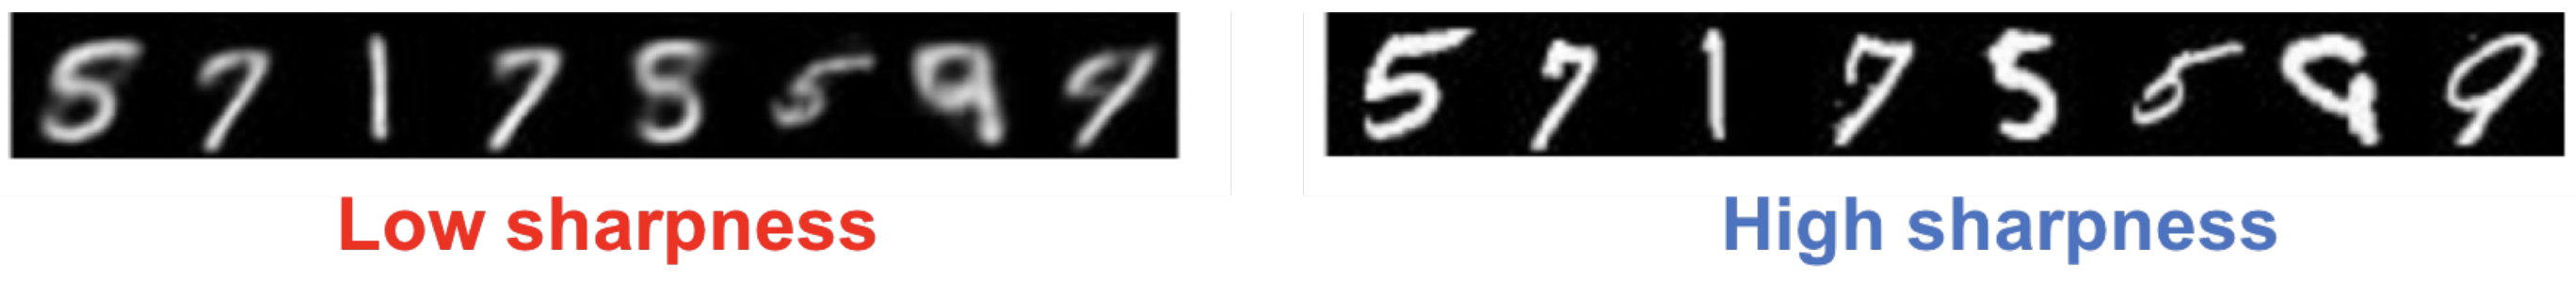
\includegraphics[width=0.9\linewidth]{figs/sharpness}
			\end{figure}
			The conditional distribution $p(y | \bx)$ should have low entropy (each image $\bx$ should have distinctly recognizable object).
			\item \textbf{Diversity}
			\begin{figure}
				\centering
				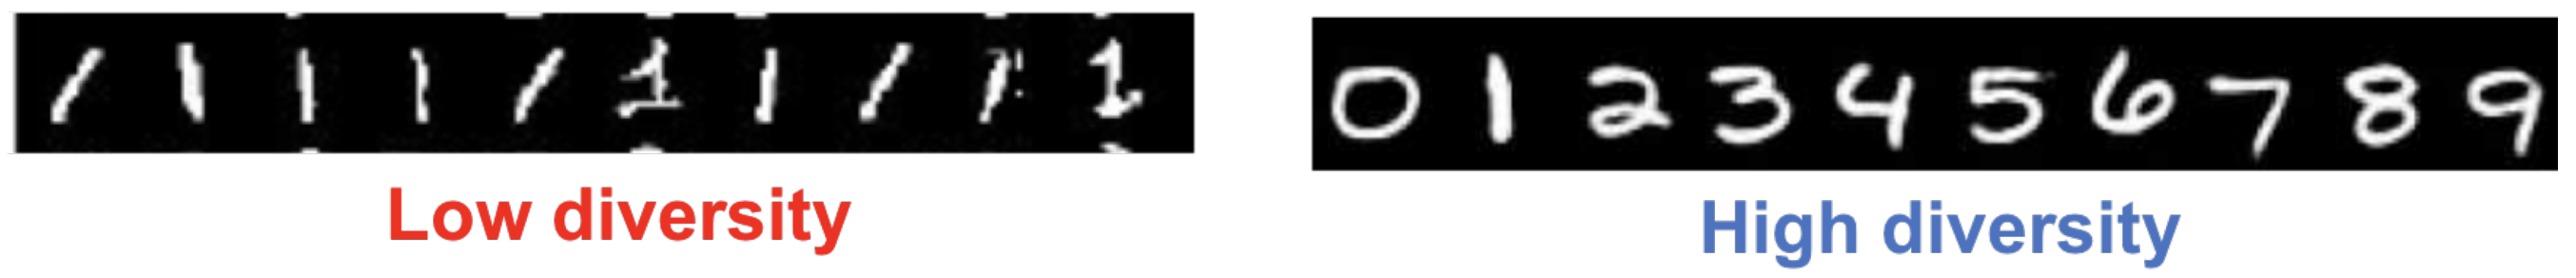
\includegraphics[width=0.9\linewidth]{figs/diversity}
			\end{figure}
			The marginal distribution $p(y) = \int p(y | \bx) p(\bx) d \bx$ should have high entropy (there should be as many classes generated as possible).
		\end{itemize}
	\end{block}
	\myfootnotewithlink{https://deepgenerativemodels.github.io}{image credit: https://deepgenerativemodels.github.io}
\end{frame}
%=======
\begin{frame}{Evaluation of likelihood-free models}
	\begin{block}{What do we want from samples?}
		\begin{itemize}
			\item \textbf{Sharpness.}
			The conditional distribution $p(y | \bx)$ should have low entropy (each image $\bx$ should have distinctly recognizable object).
			\item \textbf{Diversity.}
			The marginal distribution $p(y) = \int p(y | \bx) p(\bx) d \bx$ should have high entropy (there should be as many classes generated as possible).
		\end{itemize}
	\end{block}
	\begin{figure}
		\centering
		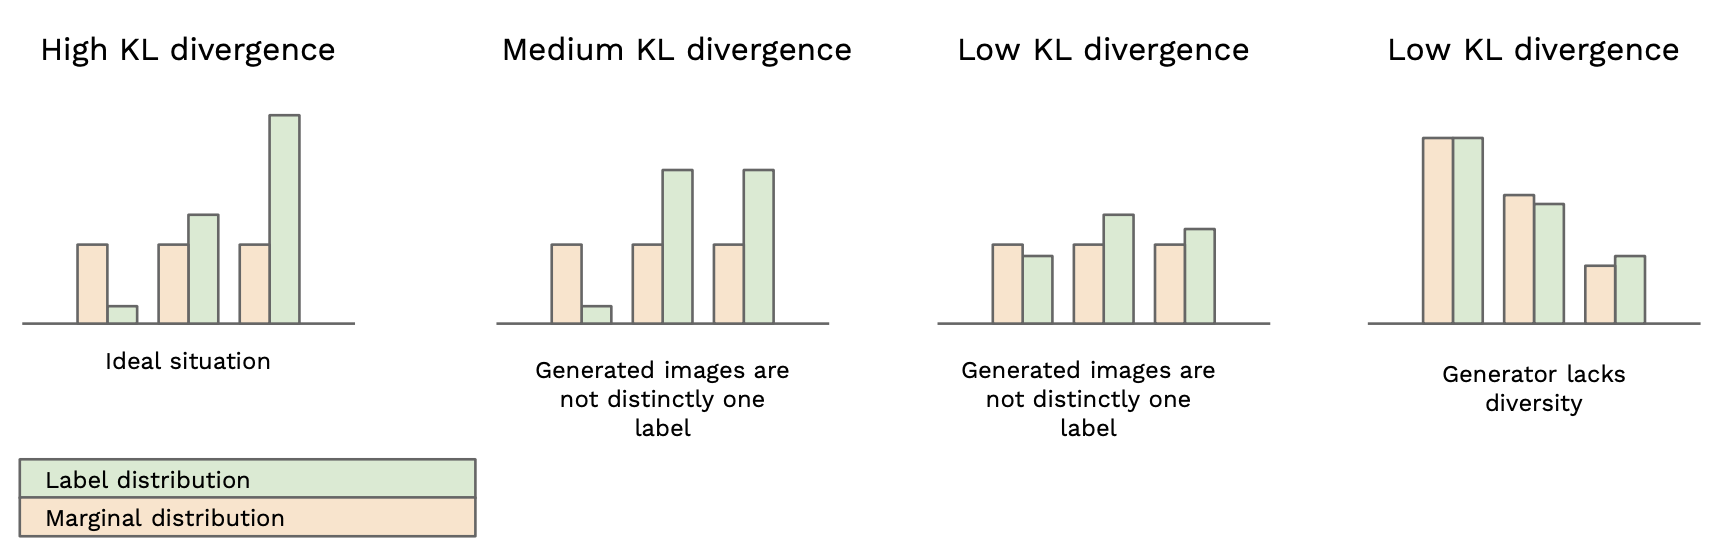
\includegraphics[width=1.0\linewidth]{figs/is_toy}
	\end{figure}
	\myfootnotewithlink{https://medium.com/octavian-ai/a-simple-explanation-of-the-inception-score-372dff6a8c7a}{image credit: https://medium.com/octavian-ai/a-simple-explanation-of-the-inception-score-372dff6a8c7a}
\end{frame}
%=======
\begin{frame}{Evaluation of likelihood-free models}
		\begin{block}{What do we want from samples?}
		\begin{itemize}
			\item Sharpness $\Rightarrow$ low $H(y | \bx) = - \sum_{y} \int_{\bx} p(y, \bx) \log p(y | \bx) d\bx$.
			\item Diversity $\Rightarrow$ high $H(y)  = - \sum_{y} p(y) \log p(y)$.
		\end{itemize}
	\end{block}
	\begin{block}{Inception Score}
		\vspace{-0.3cm}
		\footnotesize
		\begin{align*}
			IS &= \exp(H(y) - H(y | \bx)) \\ 
			&= \exp \left( - \sum_{y} p(y) \log p(y) + \sum_{y} \int_{\bx} p(y, \bx) \log p(y | \bx) d\bx\right) \\
			&= \exp \left( \sum_{y} \int_{\bx} p(y, \bx) \log \frac{p(y | \bx)}{p(y)} d\bx\right) \\ 
			&= \exp \left( \bbE_{\bx} \sum_{y} p(y | \bx) \log \frac{p(y | \bx)}{p(y)} \right) = \exp \left( \bbE_{\bx} KL(p(y | \bx) || p(y)) \right)
		\end{align*}
	\end{block}
	\myfootnotewithlink{https://arxiv.org/abs/1606.03498}{Salimans T. et al. Improved Techniques for Training GANs, 2016}
\end{frame}
%=======
\section{Inception score/FID/Precision-Recall}
%=======
\begin{frame}{Evaluation of likelihood-free models}
	\begin{block}{Theorem (informal)}
		If $\pi(\bx)$ and $p(\bx | \btheta)$ has moment generation functions then
		\vspace{-0.1cm}
		\[
			\pi(\bx) = p(\bx | \btheta) \, \Leftrightarrow \, \bbE_{\pi} \bx^k = \bbE_{p} \bx^k, \quad \forall k \geq 1.
		\]
		\vspace{-0.7cm}
	\end{block}
	This is intractable to calculate all moments.
	\begin{block}{Frechet Inception Distance}
		\vspace{-0.3cm}
		\[
			FID (\pi, p) = \| \mathbf{m}_{\pi} - \mathbf{m}_{p}\|_2^2 + \text{Tr} \left( \bSigma_{\pi} + \bSigma_p - 2 \sqrt{\bSigma_{\pi} \bSigma_p} \right)
		\]
		\vspace{-0.5cm}
	\end{block}
	\begin{itemize}
		\item Representations are outputs of intermediate layer from pretrained classification model.
		\item $\mathbf{m}_{\pi}$, $\bSigma_{\pi} $ are mean vector and covariance matrix of feature representations for real samples from $\pi(\bx)$
		\item $\mathbf{m}_{p}$, $\bSigma_p$ are mean vector and covariance matrix of feature representations for generated samples from $p(\bx | \btheta)$.
	\end{itemize} 

	\myfootnotewithlink{https://arxiv.org/abs/1706.08500}{Heusel M. et al. GANs Trained by a Two Time-Scale Update Rule Converge to a Local Nash Equilibrium, 2017}
\end{frame}
%=======
\begin{frame}{Evaluation of likelihood-free models}
	\begin{figure}
		\centering
		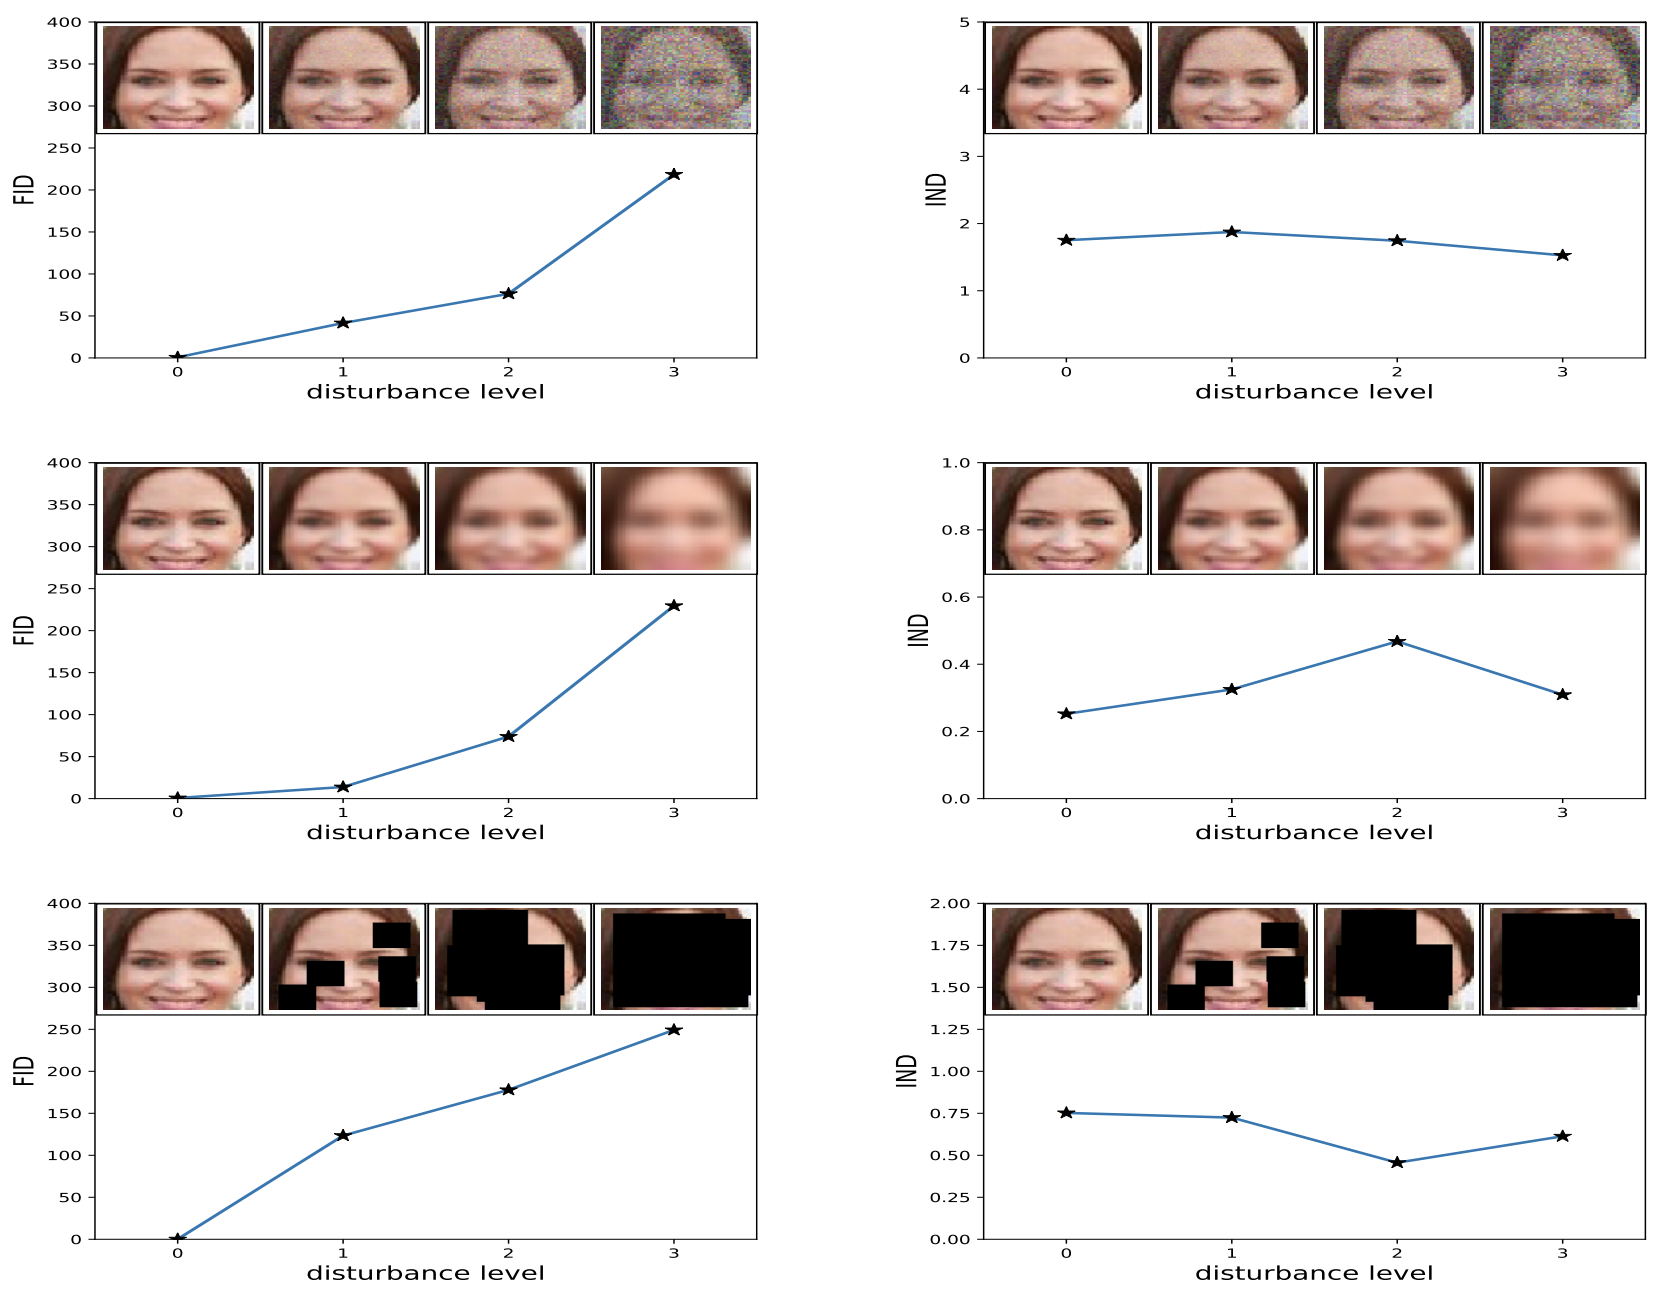
\includegraphics[width=0.9\linewidth]{figs/fid_results}
	\end{figure}
	
	\myfootnotewithlink{https://arxiv.org/abs/1706.08500}{Heusel M. et al. GANs Trained by a Two Time-Scale Update Rule Converge to a Local Nash Equilibrium, 2017}
\end{frame}
%=======
\begin{frame}{Limitations}
	\vspace{-0.5cm}
	\begin{block}{Inception Score}
		\vspace{-0.5cm}
		\[
			IS =  \exp \left( \bbE_{\bx} KL(p(y | \bx) || p(y)) \right)
		\]
		\vspace{-0.7cm}
	\end{block}
	\begin{itemize}
		\item If generator produces images with a different set of labels from the classifier training set, IS will be low.
		\item If generator produces one image per class, the IS will be perfect (there is no measure of intra-class diversity).
	\end{itemize}
	\begin{block}{Frechet Inception Distance}
		\vspace{-0.4cm}
		\[
			FID = \| \mathbf{m}_{\pi} - \mathbf{m}_{p}\|_2^2 + \text{Tr} \left( \bSigma_{\pi} + \bSigma_p - 2 \sqrt{\bSigma_{\pi} \bSigma_p} \right)
		\]
		\vspace{-0.7cm}
	\end{block}
	\begin{itemize}
		\item Needs a large sample size for evaluation.
		\item Calculation of FID is slow.
		\item Estimates only two sample moments.
	\end{itemize}
	Both scores depend on the pretrained classifier $p(y | \bx)$.

	\myfootnote{\href{https://arxiv.org/abs/1801.01973}{Barratt S., Sharma R. A Note on the Inception Score, 2018} \\
	\href{https://arxiv.org/abs/1706.08500}{Heusel M. et al. GANs Trained by a Two Time-Scale Update Rule Converge to a Local Nash Equilibrium, 2017}}
\end{frame}
%=======
\begin{frame}{Precision-Recall for Generative Models}
	\begin{block}{What do we want from samples}
		\begin{itemize}
			\item \textbf{Sharpness}: generated samples should be of high quality.
			\item \textbf{Diversity}: their variation should match that observed in the training set.
		\end{itemize}
	\end{block}
	\vspace{-0.5cm}
	\begin{figure}
		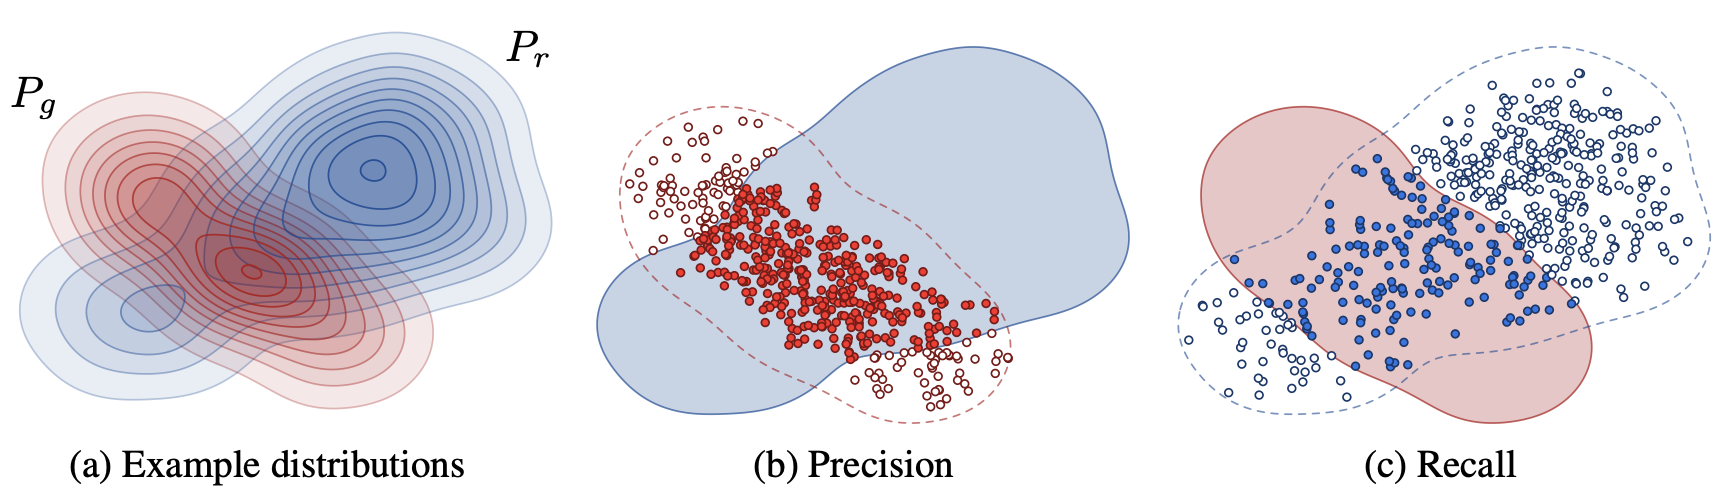
\includegraphics[width=0.95\linewidth]{figs/pr_curve}
	\end{figure}
	\vspace{-0.3cm}
	\begin{itemize}
		\item \textbf{Precision} denotes the fraction of generated images that are realistic.
		\item \textbf{Recall} measures the fraction of the training data manifold covered by the generator.
	\end{itemize}
	\myfootnotewithlink{https://arxiv.org/abs/1904.06991}{Kynkäänniemi T. et al. Improved precision and recall metric for assessing generative models, 2019}
\end{frame}
%=======
\begin{frame}{Precision-Recall for generative models}
	\begin{itemize}
		\item $\cS_{\pi} = \{\bx_i\}_{i=1}^{n} \sim \pi(\bx)$ -- real samples;
		\item $\cS_{p} = \{\bx_i\}_{i=1}^{n} \sim p(\bx | \btheta)$ -- generated samples.
	\end{itemize}
	Embed samples using pretrained classifier network (as previously):
	\[
		\cG_{\pi} = \{\mathbf{g}_i\}_{i=1}^n, \quad \cG_{p} = \{\mathbf{g}_i\}_{i=1}^n.
	\]
	Define binary function:
	\[
		f(\mathbf{g}, \cG) = 
		\begin{cases}
			1, \text{if exists } \mathbf{g}' \in \cG: \| \mathbf{g}  - \mathbf{g}'\|_2 \leq \| \mathbf{g}' - \text{NN}_k(\mathbf{g}', \cG)\|_2; \\
			0, \text{otherwise.}
		\end{cases}
	\]
	\[
		\text{Precision} (\cG_{\pi}, \cG_{p}) = \frac{1}{n} \sum_{\mathbf{g} \in \cG_{p}} f(\mathbf{g}, \cG_{\pi}); \quad \text{Recall} (\cG_{\pi}, \cG_{p}) = \frac{1}{n} \sum_{\mathbf{g} \in \cG_{\pi}} f(\mathbf{g}, \cG_{p}).
	\]
	\vspace{-0.4cm}
	\begin{figure}
		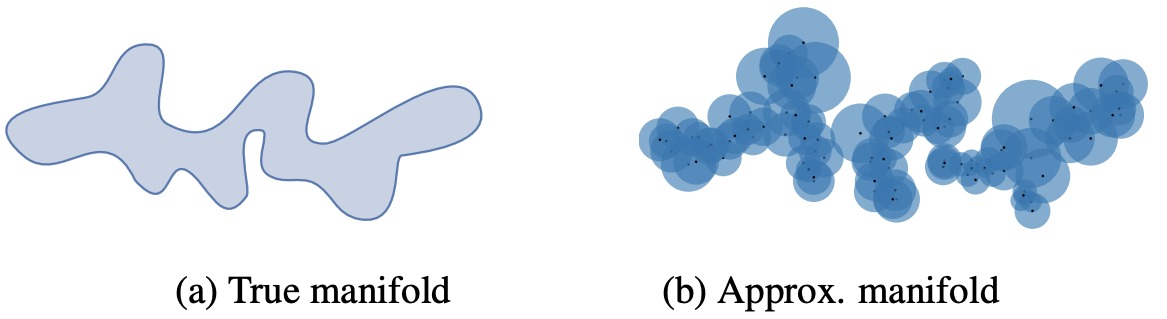
\includegraphics[width=0.7\linewidth]{figs/pr_k_nearest}
	\end{figure}
	\myfootnotewithlink{https://arxiv.org/abs/1904.06991}{Kynkäänniemi T. et al. Improved precision and recall metric for assessing generative models, 2019}
\end{frame}
%=======
\begin{frame}{Precision-Recall for generative models}
	\begin{figure}
		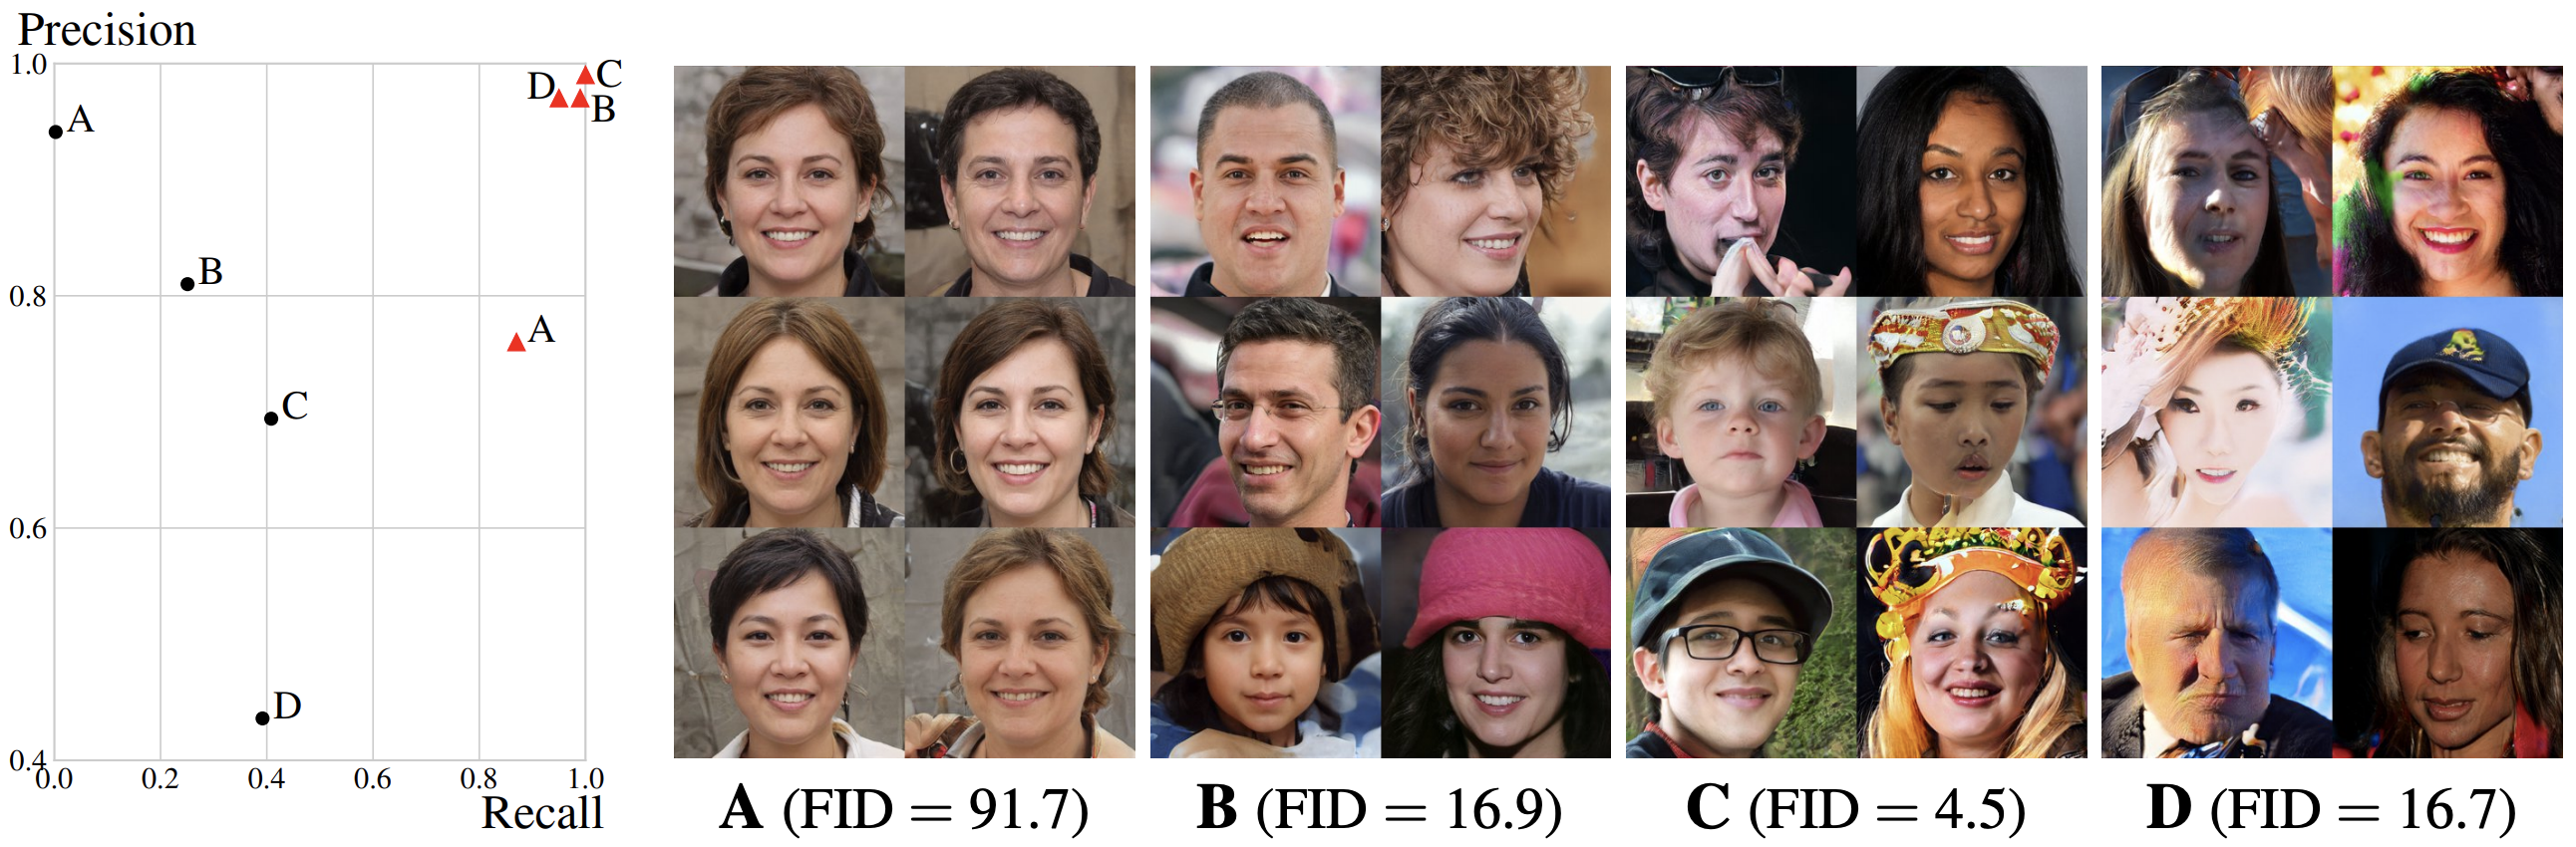
\includegraphics[width=\linewidth]{figs/pr_vs_fid}
	\end{figure}
	\begin{figure}
		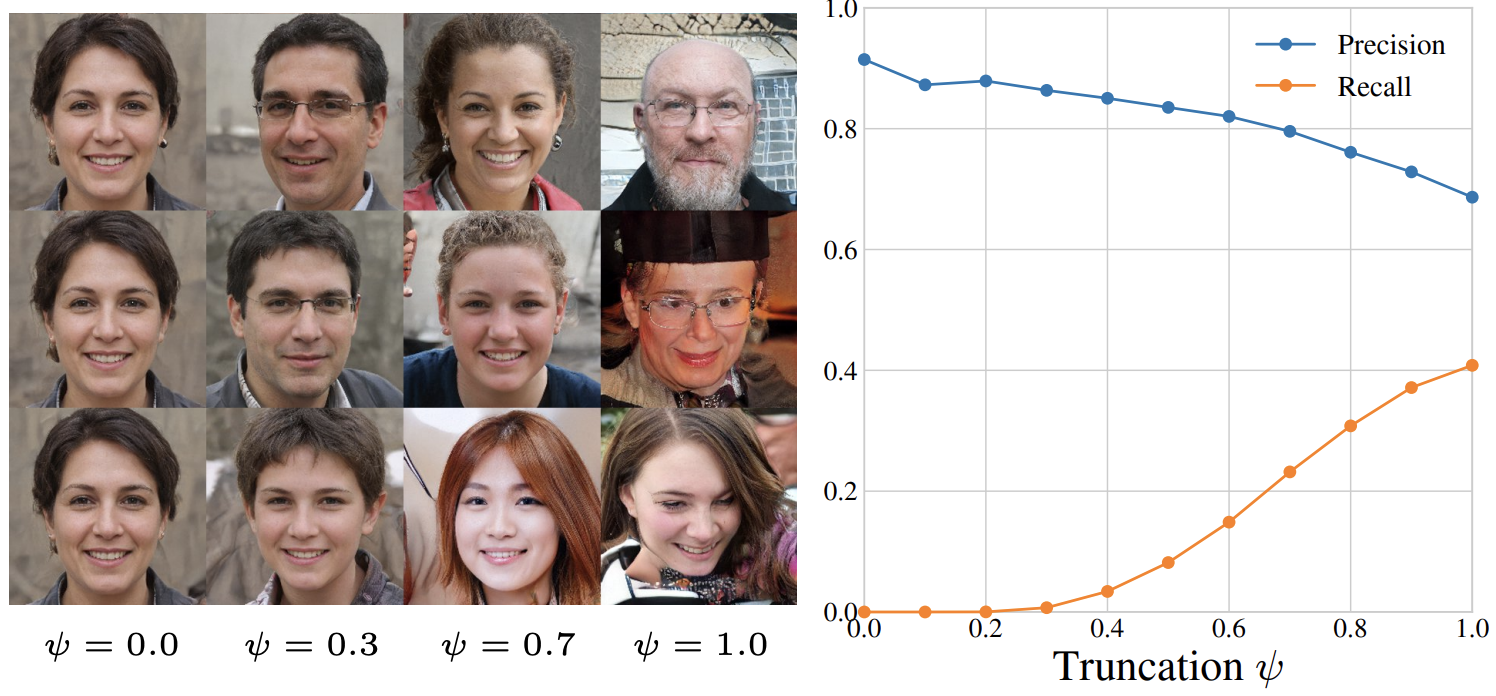
\includegraphics[width=0.75\linewidth]{figs/pr_truncation}
	\end{figure}
	\myfootnotewithlink{https://arxiv.org/abs/1904.06991}{Kynkäänniemi T. et al. Improved precision and recall metric for assessing generative models, 2019}
\end{frame}
%=======
\section{Evolution of GANs}
%=======
\begin{frame}{Evolution of GANs}
	\begin{figure}
		\centering
		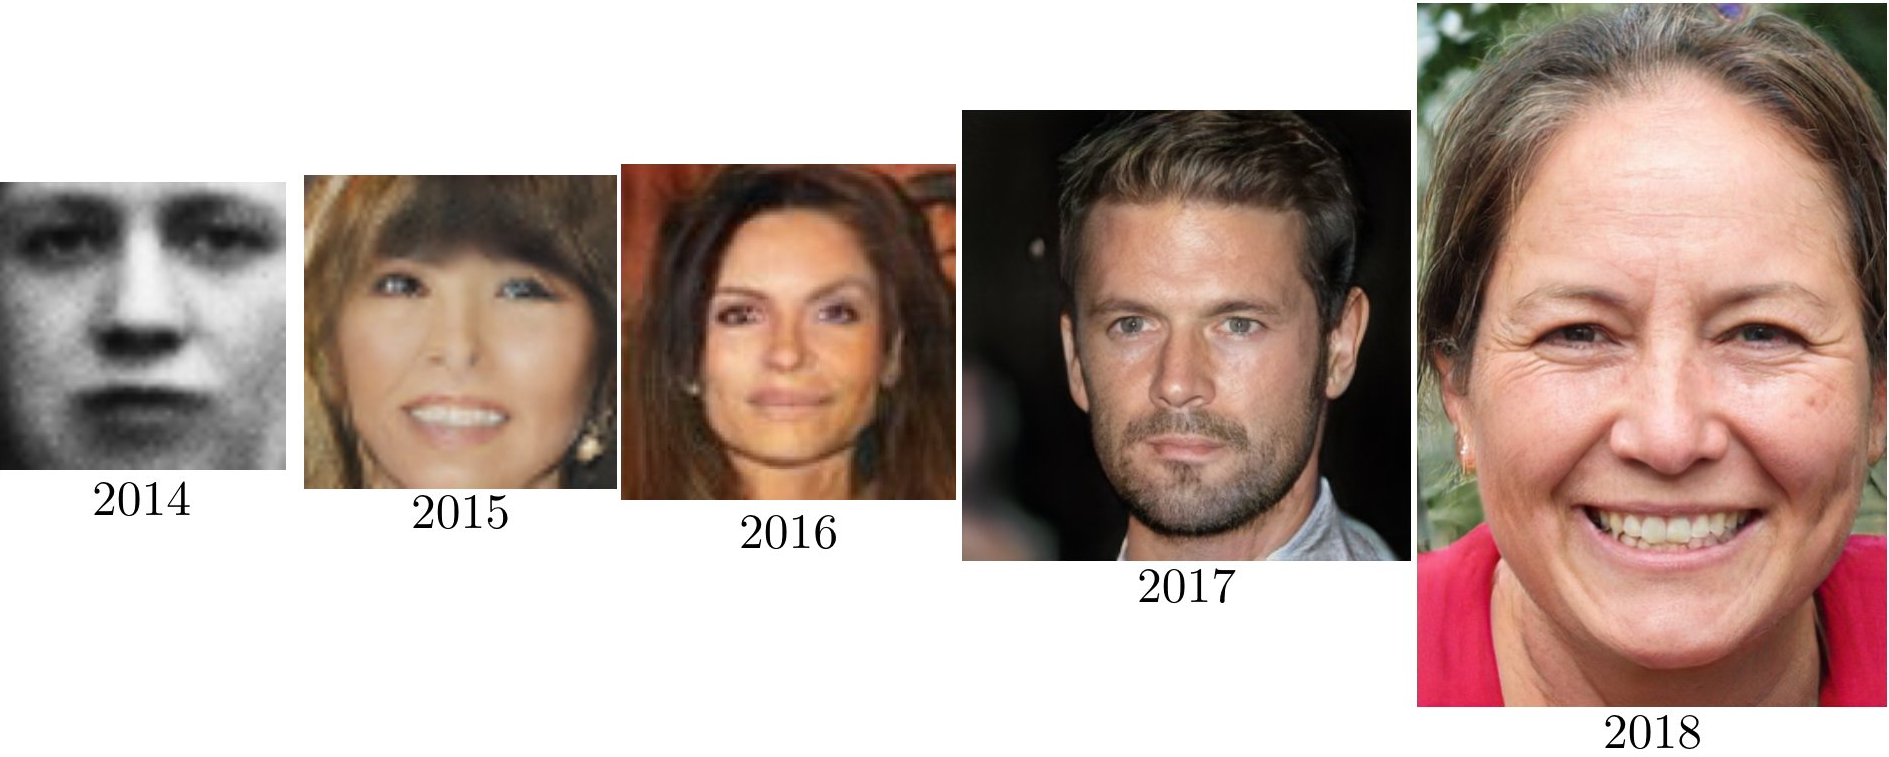
\includegraphics[width=\linewidth]{figs/gan_evolution}
	\end{figure}
	\begin{itemize}
		\item \textbf{Standard GAN} \href{https://arxiv.org/abs/1406.2661}{https://arxiv.org/abs/1406.2661}
		\item \textbf{DCGAN} \href{https://arxiv.org/abs/1511.06434}{https://arxiv.org/abs/1511.06434}
		\item \textbf{CoGAN} \href{https://arxiv.org/abs/1606.07536}{https://arxiv.org/abs/1606.07536}
		\item \textbf{ProGAN} \href{https://arxiv.org/abs/1710.10196}{https://arxiv.org/abs/1710.10196} 
		\item \textbf{StyleGAN} \href{https://arxiv.org/abs/1812.04948}{https://arxiv.org/abs/1812.04948}
	\end{itemize}
\end{frame}
%=======
\begin{frame}{Self-Attention GAN}
	Convolutional layers process the information in a local neighborhood $\Rightarrow$ inefficient for modeling long-range dependencies in images.
	\vspace{-0.3cm}
	\begin{figure}
		\centering
		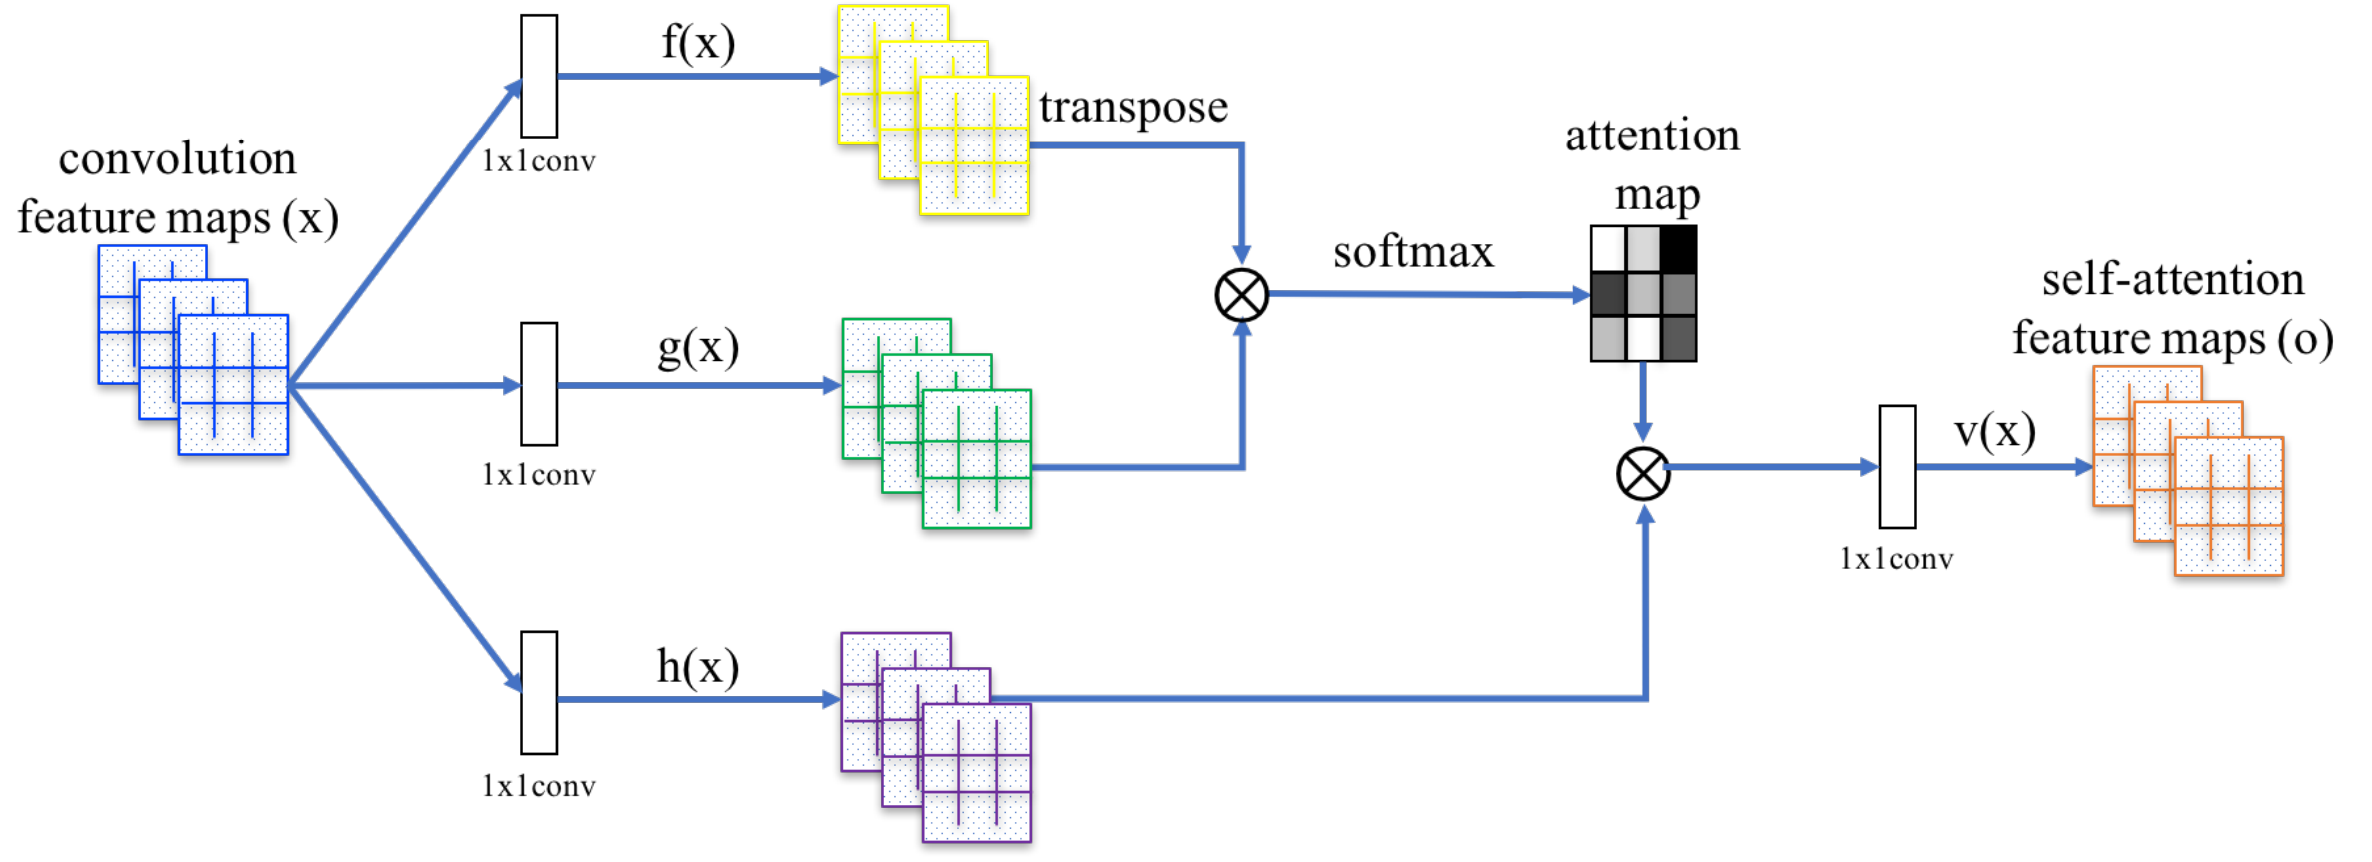
\includegraphics[width=0.9\linewidth]{figs/self-attention}
	\end{figure}
	\[
		\mathbf{f}(\bx) = \bW_f \bx, \quad \mathbf{g}(\bx) = \bW_g\bx, \quad \mathbf{h} (\bx) = \bW_h\bx, \quad \mathbf{v}(\bx) = \bW_v\bx
	\]
	\[
		s_{ij} = \mathbf{f}(\bx_i)^T \mathbf{g}(\bx_j), \quad a_{ij} = \frac{\exp{s_{ij}}}{\sum_{i=1}^N \exp{s_{ij}}}, \quad \textbf{o}_j = \textbf{v}\left( \sum_{i=1}^N a_{ij} \mathbf{h}(\bx_i) \right)
	\]
	\myfootnotewithlink{https://arxiv.org/abs/1805.08318}{Zhang H. et al. Self-Attention Generative Adversarial Networks, 2018}
\end{frame}
%=======
\begin{frame}{Self-Attention GAN}	
	\begin{block}{Convolution vs Attention}
		\vspace{-0.3cm}
		\begin{figure}
			\centering
			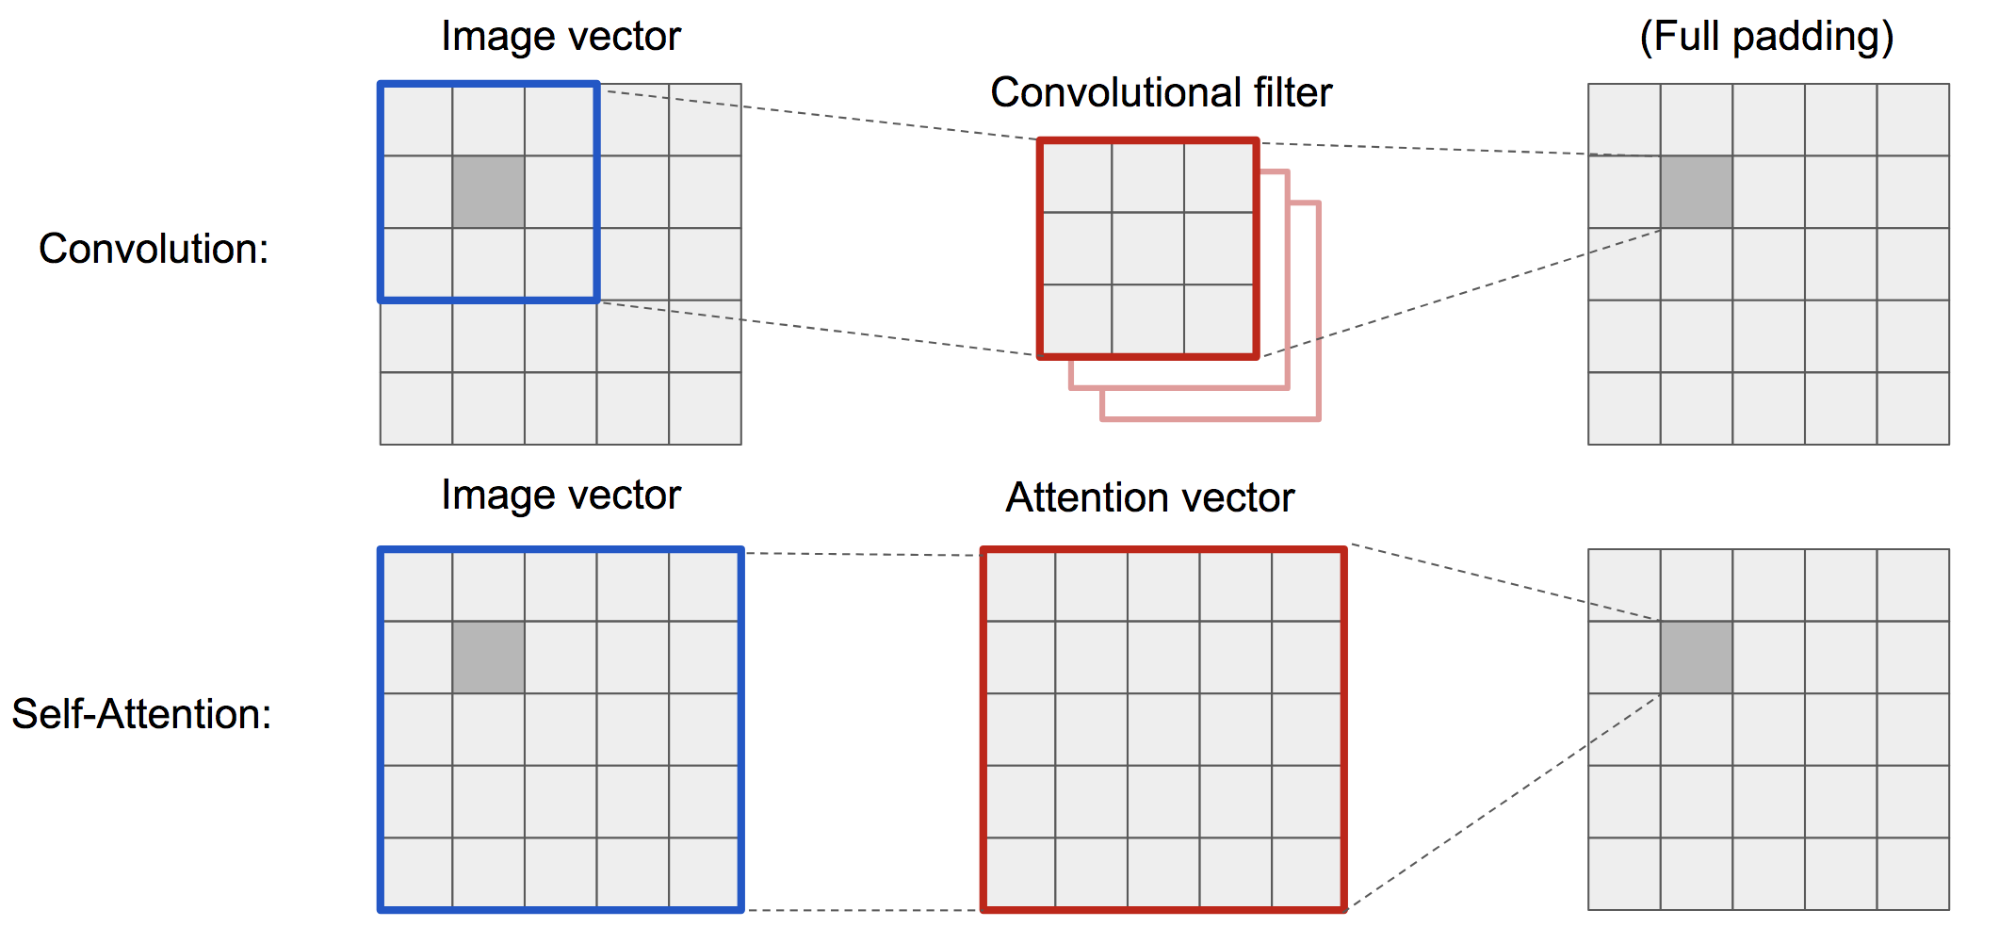
\includegraphics[width=0.7\linewidth]{figs/conv-vs-sa}
		\end{figure}
	\end{block}
	\vspace{-0.5cm}
	\begin{block}{Visualization of attention maps}
		\vspace{-0.3cm}
		\begin{figure}
			\centering
			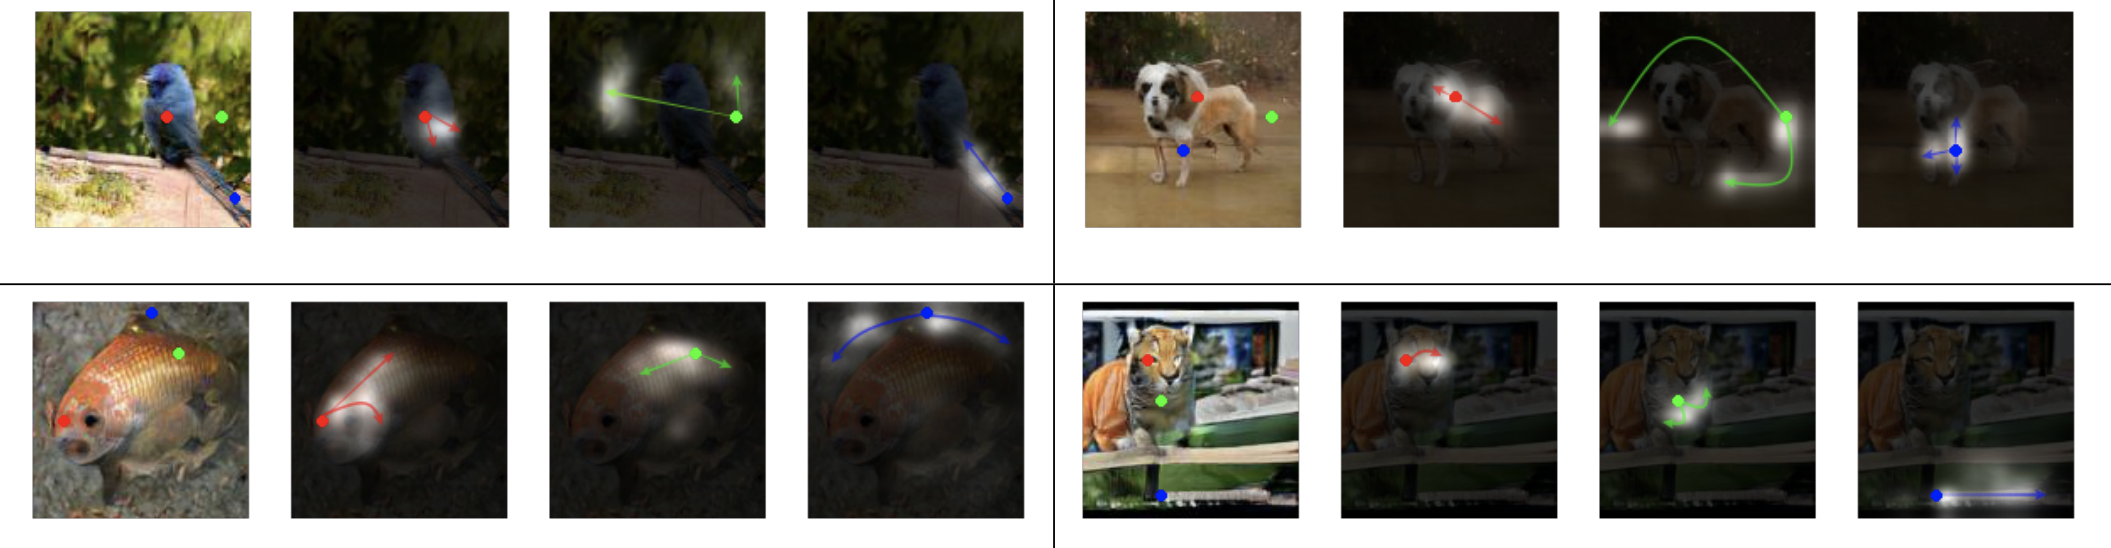
\includegraphics[width=\linewidth]{figs/sa_maps}
		\end{figure}
	\end{block}

	\myfootnote{\href{https://lilianweng.github.io/lil-log/2018/06/24/attention-attention.html}{image credit: https://lilianweng.github.io/lil-log/2018/06/24/attention-attention.html}	\\ 
	\href{https://arxiv.org/abs/1805.08318}{Zhang H. et al. Self-Attention Generative Adversarial Networks, 2018}}
\end{frame}
%=======
\begin{frame}{BigGAN}
	\begin{block}{Batch-size is matter}
		\begin{figure}
			\centering
			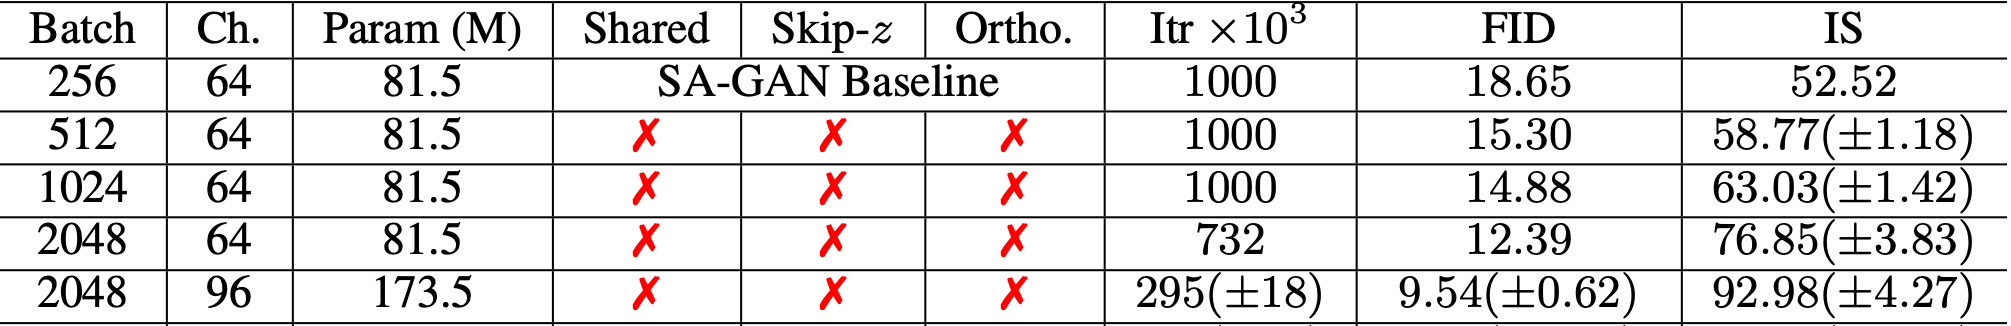
\includegraphics[width=\linewidth]{figs/biggan_results}
		\end{figure}
	\end{block}
	\begin{block}{Samples (512x512)}
		\begin{figure}
			\centering
			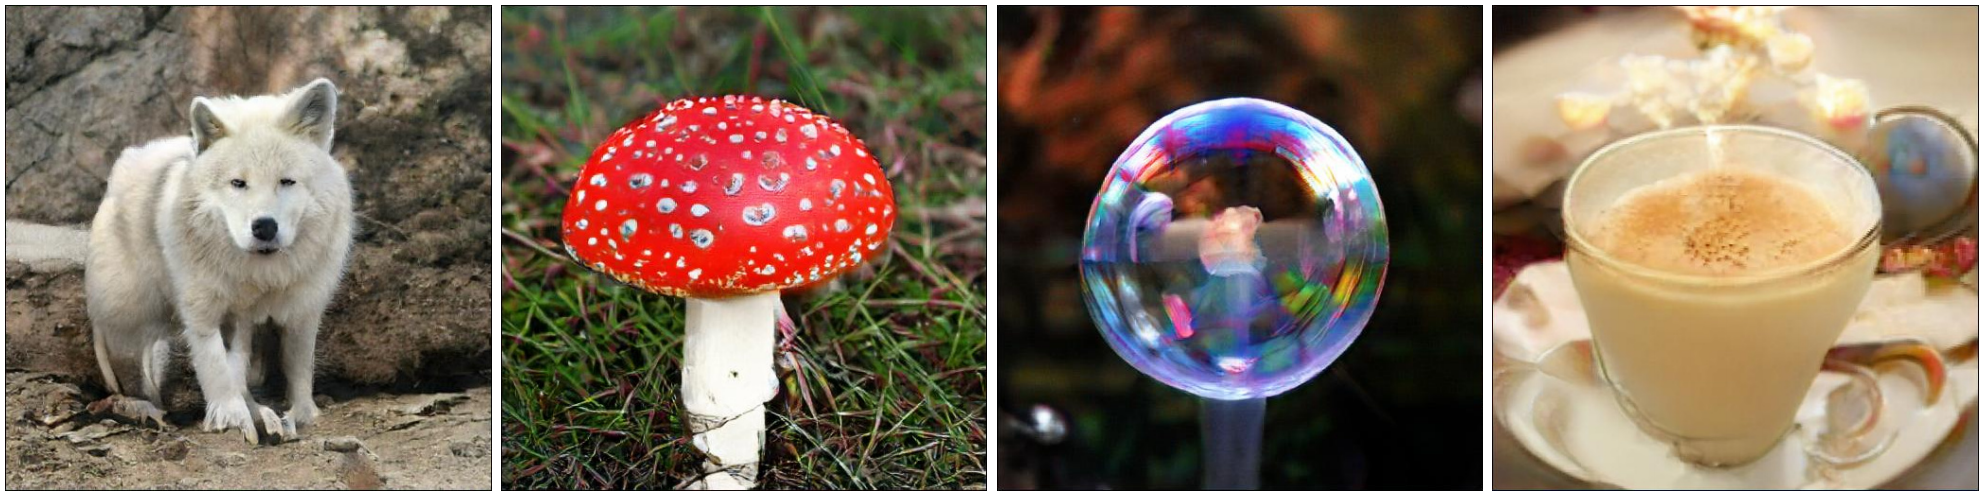
\includegraphics[width=\linewidth]{figs/biggan_samples}
		\end{figure}
	\end{block}
	\vspace{-0.4cm}
	\myfootnotewithlink{https://arxiv.org/abs/1809.11096}{Brock A., Donahue J., Simonyan K. Large Scale GAN Training for High Fidelity Natural Image Synthesis, 2018}
\end{frame}
%=======
\begin{frame}{Progressive Growing GAN}
	\begin{block}{Problems with HR image generation}
		\begin{itemize}
			\item Disjoint manifolds $\Rightarrow$ gradient problem.
			\item Small minibatch $\Rightarrow$ training instability.
		\end{itemize}
	\end{block}
	\vspace{-0.2cm}
	\begin{block}{Samples (1024x1024)}
		\vspace{-0.2cm}
		\begin{figure}
			\includegraphics[width=0.9\linewidth]{figs/pggan_samples}
		\end{figure}
	\end{block}
	\myfootnotewithlink{https://arxiv.org/abs/1710.10196}{Karras T. et al. Progressive Growing of GANs for Improved Quality, Stability, and Variation, 2017}
s\end{frame}
\begin{frame}{Progressive Growing GAN}
	Grow both the generator and discriminator progressively, new layers will introduce higher-resolution details as the training progresses. 
	\begin{itemize}
		\item Train GAN which generate 4x4 images (2 convs for G and D).
		\item Add upsampling layers to G, downsampling layers to D.
		\item Train GAN which generate 8x8 images.
		\item etc.
	\end{itemize}
	\vspace{-0.2cm}
	\begin{figure}
		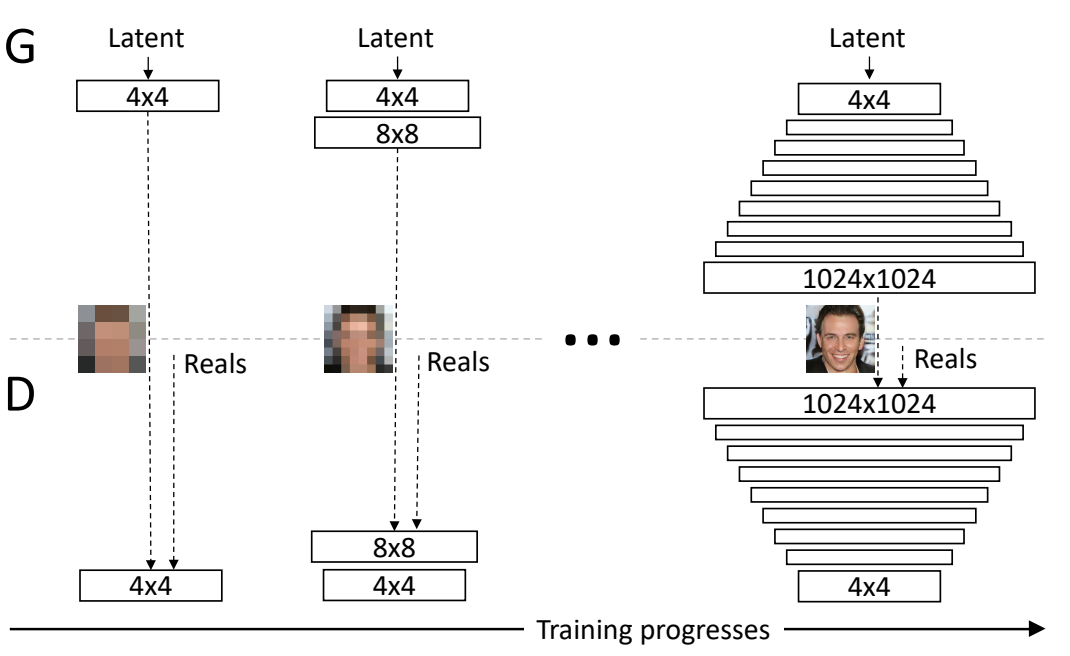
\includegraphics[width=0.75\linewidth]{figs/pggan_arch}
	\end{figure}

	\myfootnotewithlink{https://arxiv.org/abs/1710.10196}{Karras T. et al. Progressive Growing of GANs for Improved Quality, Stability, and Variation, 2017}
\end{frame}
%=======
\begin{frame}{StyleGAN}
	\begin{itemize}
		\item Generating of HR images is hard.
		\item Progressive growing greatly simplifies the task.
		\item The ability to control specific features of the generated image is very limited.
	\end{itemize}
	\begin{block}{Face image features}
		\begin{itemize}
			\item Coarse (pose, general hair style, face shape). Resolution $4^2 - 8^2$.
			\item Middle (finer facial features, hair style, eyes open/closed). Resolution $16^2 - 32^2$.
			\item Fine (color scheme (eye, hair and skin) and micro features). Resolution $64^2 - 1024^2$.
		\end{itemize}
	\end{block}
	\myfootnotewithlink{https://arxiv.org/abs/1812.04948}{Karras T., Laine S., Aila T. A Style-Based Generator Architecture for Generative Adversarial Networks, 2018}
\end{frame}
%=======
\begin{frame}{StyleGAN}
	\begin{block}{Mapping Network}
		\begin{itemize}
			\item Generator input is likely to be \textbf{disentangled}.  Each component of input vector $\bz$ should be responsible for one generative factor.
			\item Mapping network $f: \cZ \rightarrow \cW$ is used to reduce correlations between components of~$\bz$.
		\end{itemize}
		\begin{minipage}[t]{0.6\columnwidth}
			\begin{figure}
				\centering
				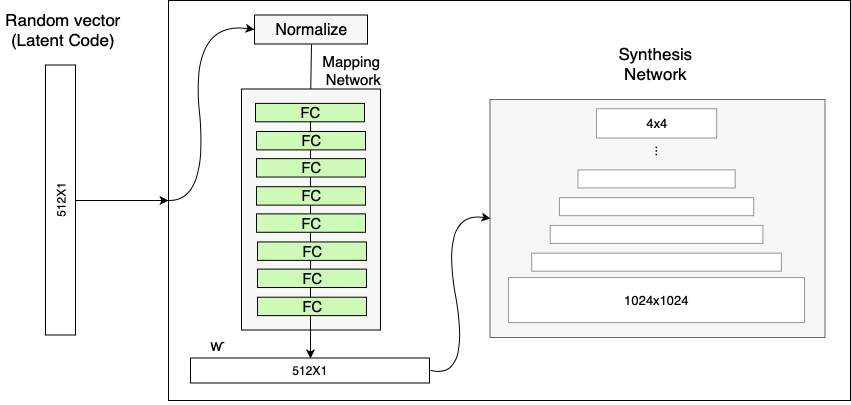
\includegraphics[width=0.98\linewidth]{figs/stylegan_mapping}
			\end{figure}
		\end{minipage}%
		\begin{minipage}[t]{0.38\columnwidth}
			\begin{figure}
				\centering
				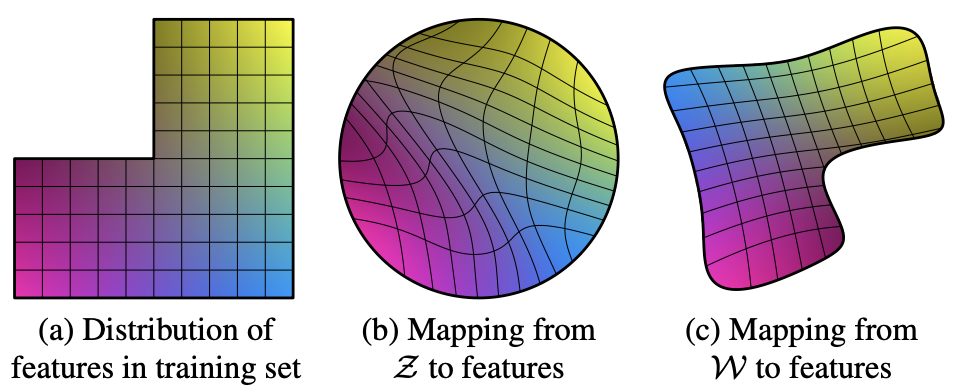
\includegraphics[width=1.0\linewidth]{figs/stylegan_curved}
			\end{figure}
		\end{minipage}
	\vspace{0.3cm}
	\end{block}

	\myfootnotewithlink{https://arxiv.org/abs/1812.04948}{Karras T., Laine S., Aila T. A Style-Based Generator Architecture for Generative Adversarial Networks, 2018}
\end{frame}
%=======
\begin{frame}{Truncation trick}
	\begin{block}{BigGAN: truncated normal sampling}
		\vspace{-0.3cm}
		\[
			p(\bz | b) = \cN(\bz | 0, 1) / \int_{-\infty}^b \cN(\bz | 0, 1) d\bz
		\]
		Components of $\bz \sim \cN(0, \bI)$ which fall outside a predefined range are resampled.
	\end{block}
	
	\begin{block}{StyleGAN}
		\vspace{-0.2cm}
		\[
			\bw' = \hat{\bw} + \psi \cdot (\bw - \hat{\bw}), \quad \hat{\bw} = \bbE_{\bz} p(f(\bz))
		\]
		\vspace{-0.2cm}
		\begin{itemize}
			\item Constant $\psi$ is a tradeoff between diversity and fidelity. 
			\item $\psi=0.7$ is used for most of the results.
			\item Truncation is done only at the low-resolution layers.
		\end{itemize}
	\end{block}

	\myfootnotewithlink{https://arxiv.org/abs/1812.04948}{Karras T., Laine S., Aila T. A Style-Based Generator Architecture for Generative Adversarial Networks, 2018}
\end{frame}
%=======
\begin{frame}{StyleGAN}
	\begin{block}{Truncation trick}
		\begin{figure}
			\centering
			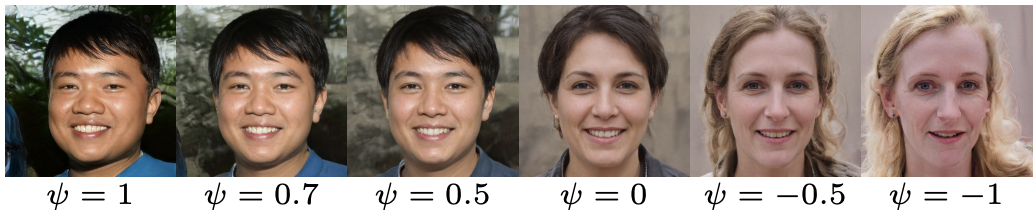
\includegraphics[width=0.85\linewidth]{figs/stylegan_truncation}
		\end{figure}
		\vspace{-0.4cm}
	\end{block}
	\begin{block}{Samples (1024x1024)}
		\begin{figure}
			\centering
			\includegraphics[width=0.8\linewidth]{figs/stylegan_samples}
		\end{figure}
	\end{block}

	\myfootnotewithlink{https://arxiv.org/abs/1812.04948}{Karras T., Laine S., Aila T. A Style-Based Generator Architecture for Generative Adversarial Networks, 2018}
\end{frame}
%=======
\begin{frame}{Summary}
	\begin{itemize}
		\item Inception Score and Frechet Inception Distance are the common metrics for GAN evaluation, but both of them have drawbacks.
		\vfill
		\item Precision-recall allows to select model with compromise with sample quality and sample diversity.	\item Self-Attention GAN allows to make huge receptive field and reduce convolution inductive bias.
		\vfill
		\item BigGAN shows that large batch size increase model quality gradually.
		\vfill
		\item Progressive growing for GAN learning allows to make training more stable.
		\vfill
		\item StyleGAN introduces mapping network to get more disentangled latent representation.
	\end{itemize}
\end{frame}
\end{document} 